Il seguente codice MatLab contiene la soluzione dell'$Es 3$:\\\
	\lstinputlisting[language=Matlab]{Cap_6/Es_3/Es_3.m}
nel qualche viene richiamato:\\\
	\begin{enumerate}
		\item \textbf{A = sparceMatrix(n)}\\\
			Effettua la creazione di \textit{matrici sparse} della dimensione $nXn$;\\\
		\item \textbf{x,i,B = jacobi(A,b,tol)}\\\
			Effettua sia il calcolo del \textit{vettore incognite} della matrice $A$, sia il numero di iterazioni impiegate, sia il calcolo di una matrice $B$ contenente il \textit{passo di ogni iterazione} con il corrispettivo \textit{valore della norma}, avendo come \textit{Input}, oltre la 	\textit{matrice}, il \textit{vettore termini noti}, e la \textit{tolleranza}, anche un \textit{vettore iniziale, in questo caso nullo}.\\\
			\lstinputlisting[language=Matlab]{Cap_6/Es_3/jacobi.m}
	\end{enumerate}
e restituisce graficamente i seguenti risultati:\\\
	\begin{figure}[H]
		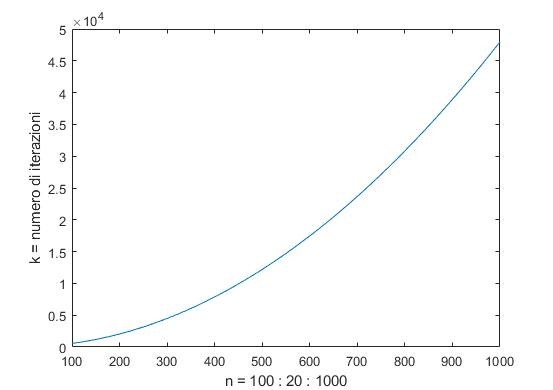
\includegraphics[width=\textwidth]{Plot/Cap_6_Es_3}
	\end{figure}